\documentclass[border=3pt]{standalone}
\usepackage{amsmath}\usepackage{amssymb}
\usepackage{fontspec}\setsansfont{Arial}\renewcommand{\familydefault}{\sfdefault}
\usepackage{tikz}
\usetikzlibrary{arrows.meta,positioning,calc,fit,backgrounds,shapes.geometric}
\definecolor{titlegray}{HTML}{5F6B78}\definecolor{ent}{HTML}{7B8794}
\definecolor{fo}{HTML}{5AA9C4}\definecolor{ho}{HTML}{2E6B86}
\definecolor{inf}{HTML}{D98A3D}\definecolor{vio}{HTML}{9B86C4}
\definecolor{smac}{HTML}{2E8AA6}\definecolor{kgc}{HTML}{E7B15A}
\definecolor{fillteal}{HTML}{E3EEF2}\definecolor{fillamber}{HTML}{FBF0E2}
\definecolor{fillgrey}{HTML}{F1F3F5}\definecolor{fillviolet}{HTML}{EFEAF6}
\definecolor{inkmid}{HTML}{3D4751}\definecolor{distract}{HTML}{B3403A}
\begin{document}
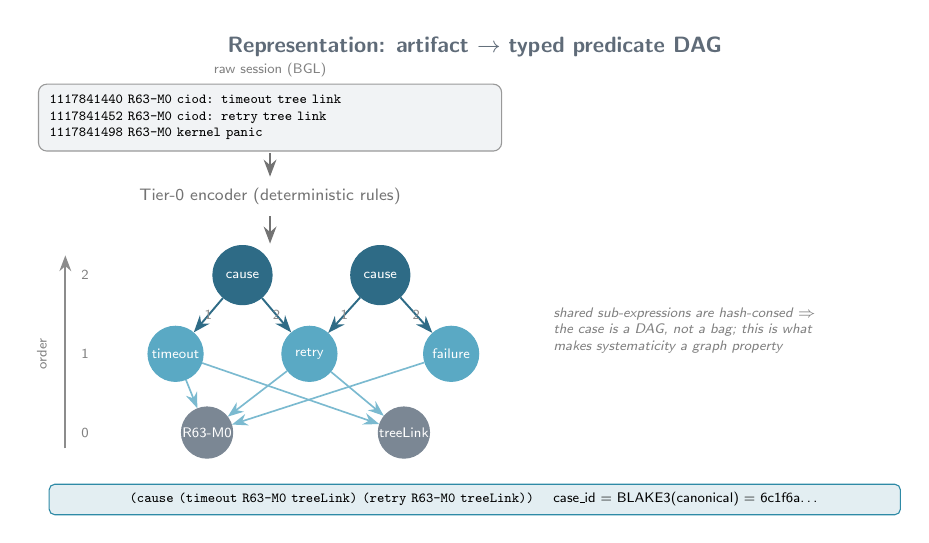
\begin{tikzpicture}[
  font=\sffamily,>=Stealth,
  ttl/.style={font=\sffamily\fontsize{8}{9}\selectfont\bfseries, color=titlegray, align=center},
  sub/.style={font=\sffamily\fontsize{6}{7}\selectfont, color=black!55, align=center},
  micro/.style={font=\sffamily\fontsize{5.2}{6}\selectfont, color=black!50, align=center},
  enode/.style={circle, draw=ent, fill=ent, text=white, font=\sffamily\fontsize{5.2}{6}\selectfont, inner sep=0pt, minimum size=6.5mm, align=center},
  fnode/.style={circle, draw=fo, fill=fo, text=white, font=\sffamily\fontsize{5.2}{6}\selectfont, inner sep=0pt, minimum size=7mm, align=center},
  hnode/.style={circle, draw=ho, fill=ho, text=white, font=\sffamily\fontsize{5.2}{6}\selectfont, inner sep=0pt, minimum size=7.5mm, align=center},
  pbox/.style={rounded corners=2pt, draw, align=center, inner sep=3pt, font=\sffamily\fontsize{6}{7}\selectfont},
  flowarr/.style={->, line width=0.7pt, color=black!55},
  horel/.style={->, line width=0.7pt, color=ho},
  forel/.style={->, line width=0.6pt, color=fo!80},
]

\node[ttl] at (5.5,5.6) {Representation: artifact $\rightarrow$ typed predicate DAG};
\node[draw=black!40,fill=fillgrey,rounded corners=3pt,align=left,inner sep=4pt,font=\ttfamily\fontsize{5}{6}\selectfont,text width=5.6cm] (log) at (2.9,4.7) {1117841440 R63-M0 ciod: timeout tree link\\1117841452 R63-M0 ciod: retry tree link\\1117841498 R63-M0 kernel panic};
\node[micro] at (2.9,5.3) {raw session (BGL)};
\node[sub] (enc) at (2.9,3.7) {Tier-0 encoder (deterministic rules)};
\draw[flowarr] (2.9,4.25)--(2.9,3.95); \draw[flowarr] (2.9,3.45)--(2.9,3.1);
% order axis
\draw[->,line width=0.6pt,color=black!45] (0.3,0.5) -- (0.3,2.95);
\node[micro,rotate=90] at (0.0,1.7) {order};
\foreach \o/\y in {0/0.7,1/1.7,2/2.7} {\node[micro] at (0.55,\y) {\o};}
\node[enode] (e1) at (2.1,0.7) {R63-M0}; \node[enode] (e2) at (4.6,0.7) {treeLink};
\node[fnode] (f1) at (1.7,1.7) {timeout}; \node[fnode] (f2) at (3.4,1.7) {retry}; \node[fnode] (f3) at (5.2,1.7) {failure};
\node[hnode] (h1) at (2.55,2.7) {cause}; \node[hnode] (h2) at (4.3,2.7) {cause};
\foreach \h/\a/\i in {h1/f1/1,h1/f2/2,h2/f2/1,h2/f3/2} {\draw[horel] (\h)--(\a) node[midway,font=\sffamily\fontsize{4.4}{5}\selectfont,color=black!45,inner sep=1pt]{\i};}
\foreach \f/\e in {f1/e1,f1/e2,f2/e1,f2/e2,f3/e1} {\draw[forel] (\f)--(\e);}
\node[micro,align=left,text width=3.6cm] at (8.3,2.0) {\textit{shared sub-expressions are hash-consed $\Rightarrow$ the case is a DAG, not a bag; this is what makes systematicity a graph property}};
\node[pbox,draw=smac,fill=fillteal,text=black,font=\sffamily\fontsize{5.2}{6.2}\selectfont,text width=10.6cm] at (5.5,-0.15) {\texttt{(cause (timeout R63-M0 treeLink) (retry R63-M0 treeLink))} \quad case\_id = BLAKE3(canonical) = 6c1f6a\ldots};

\end{tikzpicture}
\end{document}
